%\documentclass[handout]{beamer}
\documentclass[cjk,usenames,dvipsnames]{beamer}
%\usepackage[table]{xcolor}
\usepackage{pgf}
\usepackage{pgf,pgfarrows,pgfnodes,pgfautomata,pgfheaps,pgfshade}
\usepackage{beamerthemesplit}
\usepackage{xcolor,colortbl}
\usepackage{amsmath}
\usepackage{graphicx}
%\usepackage{pdfsync}
\usepackage{xspace}
\usepackage{subfigure}
%\usepackage{subcaption}
%\usepackage{subfig}
\usepackage{amsmath,amsfonts,amssymb}
\usepackage{comment}
\useoutertheme{smoothbars}
\usepackage{longtable}
\usepackage{float}
\usepackage{rotating}
\usepackage{rotfloat}
\usepackage{booktabs}
\usepackage[small,bf]{caption}
\usepackage{dsfont}
\usepackage{hyperref}
\usepackage{tikz}
\usepackage{latexsym}
\usepackage{amsmath}
\usepackage{amssymb}
\usepackage{bm}
\usepackage{graphicx}
\usepackage{wrapfig}
\usepackage{fancybox}
\usepackage{mathtools}
\usetikzlibrary{decorations.pathreplacing}


%\usetheme{Frankfurt}
%\usetheme{Madrid}
%\usetheme{Singapore}
\usetheme{Berlin}
%\usetheme{Boadilla}
%\usetheme{Ilmenau}

\newcommand{\backupbegin}{
   \newcounter{finalframe}
   \setcounter{finalframe}{\value{framenumber}}
}
\newcommand{\backupend}{
   \setcounter{framenumber}{\value{finalframe}}
}

\newcolumntype{g}{>{\columncolor{blue!15}}c}
\newcolumntype{y}{>{\columncolor{YellowGreen!25}}c}
\newcommand{\blist}{\begin{trivlist}{}}
\newcommand{\elist}{\end{trivlist}}
\newcommand{\beqb}{\begin{eqnarray*}}
\newcommand{\eeqb}{\end{eqnarray*}}
\def\bline{\vskip 16pt}
\def\Tiny{ \font\Tinyfont = cmr10 at 6pt \relax  \Tinyfont}

\makeatletter
  \newcommand\tinyv{\@setfontsize\tinyv{4pt}{5}}
\makeatother

\definecolor{beep}{rgb}{0,0,1.0}
\definecolor{Gray}{gray}{0.8}
\definecolor{myRed}{gray}{0.8}

\beamertemplateshadingbackground{red!01}{blue!01}

%: Beamer commands

%% This command generates a TOC after each section;
%%  I have placed it AFTER the first section
%\AtBeginSection[] % Displays outline at start of each section
%{
%  \begin{frame}<beamer>{Outline}
%    \tableofcontents[currentsection,currentsection]
%  \end{frame}
%}
%\setbeamertemplate{caption}[numbered] % Figures and Tables are numbered
%\setbeamertemplate{navigation symbols}{} % Navigation symbols are not displayed
%\setbeamertemplate{frametitle}[default][center] % Centers the title of the frame
%\setbeamercolor*{alerted text}{fg=blue}
%%\setbeamerfont{alerted text}{series=\bfseries}


% The next command changes the footer a little bit -- removes the () after authors
\makeatletter
\setbeamertemplate{footline}
{
  \leavevmode%
  \hbox{%
  \begin{beamercolorbox}[wd=.333333\paperwidth,ht=2.25ex,dp=1ex,center]{author in head/foot}%
    \usebeamerfont{author in head/foot}\insertshortauthor%~~(\insertshortinstitute)
  \end{beamercolorbox}%
  \begin{beamercolorbox}[wd=.333333\paperwidth,ht=2.25ex,dp=1ex,center]{title in head/foot}%
    \usebeamerfont{title in head/foot}\insertshorttitle
  \end{beamercolorbox}%
  \begin{beamercolorbox}[wd=.333333\paperwidth,ht=2.25ex,dp=1ex,right]{date in head/foot}%
    \usebeamerfont{date in head/foot}\insertshortdate{}\hspace*{2em}
    \insertframenumber{} / \inserttotalframenumber\hspace*{2ex}
  \end{beamercolorbox}}%
  \vskip0pt%
}

% I changed the color of the first box in the footer to match the third for symmetry
\setbeamercolor*{author in head/foot}{parent=palette primary}


% I increased the space between list items
% The original settings are in the file: ``beamerbaselocalstructure.sty'', in the folder ``base''
\def\@listi{\leftmargin\leftmargini
            \topsep 3\p@ \@plus2\p@ \@minus2.5\p@
            \parsep 2\p@
            \itemsep9\p@ \@plus6\p@ \@minus9\p@}
\let\@listI\@listi
\def\@listii{\leftmargin\leftmarginii
              \topsep    2\p@ \@plus1\p@ \@minus2\p@
              \parsep    1\p@   \@plus\p@
              \itemsep6\p@ \@plus4\p@ \@minus6\p@}
\def\@listiii{\leftmargin\leftmarginiii
              \topsep    2\p@ \@plus1\p@ \@minus2\p@
              \parsep    1\p@   \@plus\p@
              \itemsep6\p@ \@plus4\p@ \@minus6\p@}

% Changed theorem settings to add numbering and remove font change of header
\setbeamertemplate{theorem begin}
{%
\begin{\inserttheoremblockenv}
{%
%\inserttheoremheadfont
\inserttheoremname
\inserttheoremnumber
\ifx\inserttheoremaddition\@empty\else\ (\inserttheoremaddition)\fi%
%\inserttheorempunctuation
}%
}
\setbeamertemplate{theorem end}{\end{\inserttheoremblockenv}}

\makeatother

%\renewcommand{\emph}[1]{\textcolor{red}{\textit{#1}}}
\renewcommand{\emph}[1]{\textcolor{red}{#1}}

%\setcounter{tocdepth}{2}


% PREAMBLE ENDS HERE (end)


\begin{document}


\title[\tiny Green innovation measure using word2vec]
{\large Green innovation measure using word2vec}

\author[\tiny Tuhin Harit and Serena Xiao]
{Tuhin Harit and Serena Xiao \\
}

\institute[UTD]
{University of Texas at Dallas }

\date[\today]


\begin{frame}
	\titlepage
\end{frame}

\section{Introduction}


\begin{frame}{Introduction}

\begin{itemize}
    \item large fund flow into environmental, social and governance, i.e. ESG funds
    \item Existing literature seems to lack a good "green-innovation" proxy measure which unambiguously captures green innovation leading to ambiguous firm performance prediction
    \item Existing sentiment analysis papers (before Li et al) typically used manually constructed dictionaries
    \item Using Word2vec (i et al 2020) we create a green innovation sentiment dictionary that learns from the training set
    \item Using dictionary we create Green innovation score and find that it significantly predicts the "actual" green innovation by firms
\end{itemize}


\end{frame}



\begin{frame}{Existing literature}

 
  \begin{itemize}

    \item increasing number of empirical studies exploring the relationship between firm performances and green innovation (Lee et al 2015, Driessan et al 2013, Albino et al 2012 etc)
       \item Results are mixed - remains ambiguous how or whether the adoption of green innovation would affect a firm's performance
       \item \textbf{obstacle}: lack of consistent definition and measure of \textbf{green innovation}
       \item our contribution: create a green innovation measure using word2vec
  \end{itemize}

\end{frame}

\section{Data and Methodology}

\begin{frame}{Data}
Sample includes firms with past ESG shareholder proposals ("Green Firms").\\
R\&D exp in these firms represents "True" green innovation.
\begin{itemize}
    \item Review ~14500 transcripts ~450 firms covering period of 2005-2020
    \item Develop alternate L\&M green innovation - hand-crafted dictionary seeded with most frequently occurring words derived from authoritative texts
    \item  We do TF, TF-IDF (captures a word's relevance to a document in a collection of documents) and log TF-IDF
\end{itemize}

\end{frame}

\begin{frame}{Methodology}


  \begin{itemize}
    \item follow the procedure adopted in Li et al. (2020) to calculate the word embedding vectors and construct scoring system 
    \item word2vec - technique for natural language processing, which uses a neural network model to learn the word associations
         \item ultimate goal of the model is to predict neighboring words given an word input
         \end{itemize}
        
  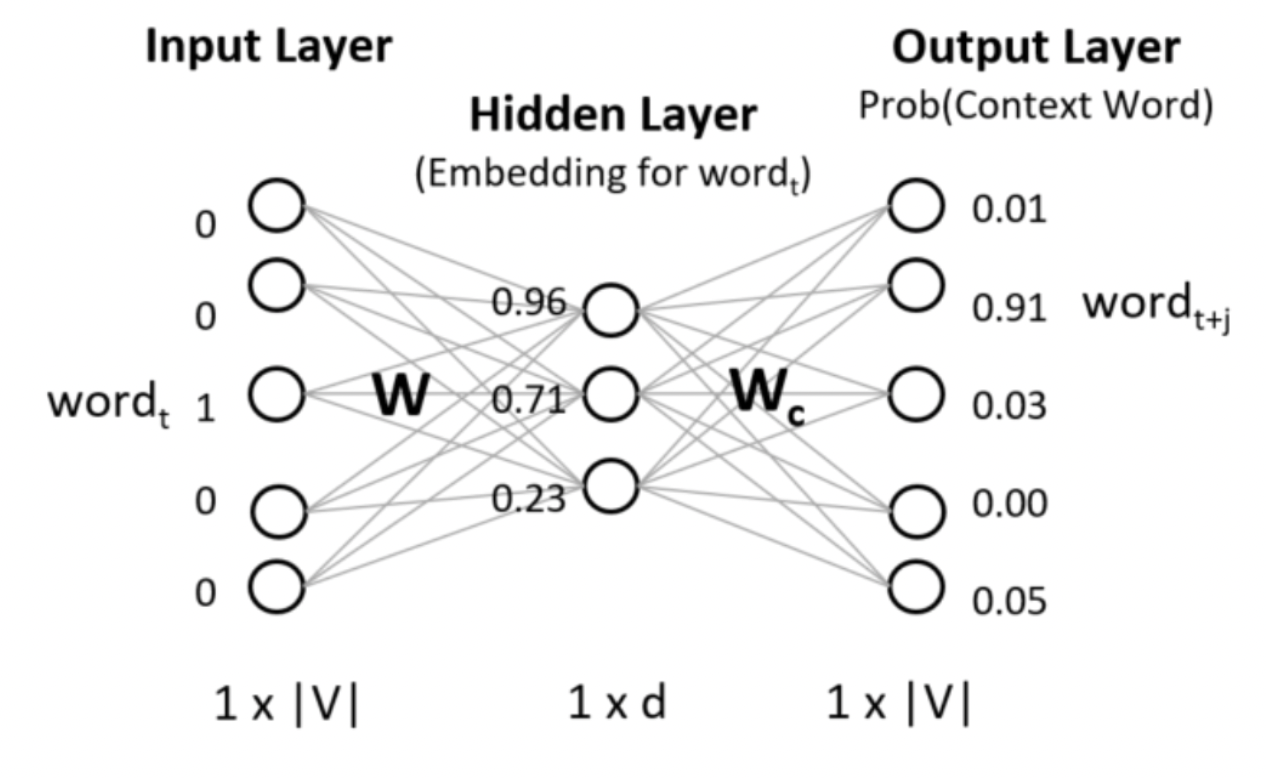
\includegraphics[height=3cm, width=8cm]{word2vec.png}

\end{frame}

\begin{frame}{Methodology}


  \begin{itemize}

    \item consider a word as neighbor if it is within five words from a given word 
    \item a word embedding coverts to a 100-dimensional vector that represents the meaning of the word (dimension = 100)
    \item use cosine similarity to quantify distance between two words 
         \end{itemize}
        
  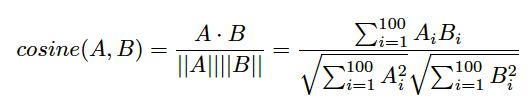
\includegraphics[height=2cm, width=8cm]{cosine.png}

\end{frame}

\begin{frame}{Methodology}

  \begin{itemize}

    \item use bootstrapping to construct \textbf{green innovation} dictionary 
    \item calculate score for each transcript:
    \begin{itemize}
        \item raw score: frequency of dictionary words normalized by the total number of words
        \item TF-IDF: multiply word frequency in a document with the inverse document frequency of a word 
        \item TF-IDF with log normalization
    \end{itemize}
    \item output - green innovation score for each transcript 
    \item Alternate measure (L\&M) generates seed words from authoritative research paper(E.g. Chen et al 2008) and books (e.g. Carbon Footprinting by Muthu)
         \end{itemize}
\end{frame}

\section{Results}

\begin{frame}{Results - dictionary comparison with alternative method}

  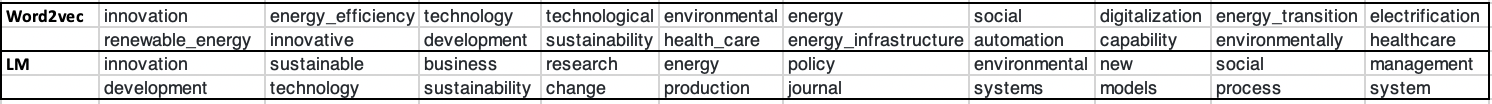
\includegraphics[height=2cm, width=11cm]{dict.png}

  \begin{itemize}
    \item only 10 common words that appear in the top 60 words in both dictionaries (16.7\%) 
    \item L\&M dictionary involves many general words that are not closely tied to green innovation, such as
"value", "role", "case", etc
         \end{itemize}
\end{frame}


\begin{frame}{Results - validation}

  \begin{itemize}
  \begin{scriptsize}
    \item evaluate whether the scores truly capture the R&D effort and overall company strategy related to green
innovation 
    \item validate our results by using R\&D expenses in the Compustat database
    \item both the contemporaneous and one-quarter lagged green innovation scores based on are \textbf{significantly positively} correlated with the R\&D expenses
    \item The results are equally significant for TF and WF-IDF.
    \end{scriptsize}
         \end{itemize}
\begin{figure}
	\centering
  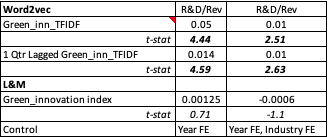
\includegraphics[height=4cm, width=7cm]{validation.png}
\end{figure}         
\end{frame}

\section{Conclusion}
\begin{frame}{Conclusion}
\begin{itemize}
    \item We are able to extend Li et al (2020) results and create an effective green innovation
    \item Our measure is more effective in capturing green innovation than traditional L\&M measure.
    \item In future, we would like to test our measure on more direct actual green innovation proxy (such as green patents).
    \item We would like to expand our dataset to include all firms
    \item A natural extension is to use this measure to predict company performance.
\end{itemize}
\end{frame}



\end{document} 